% Created 2019-08-27 mar 16:52
\documentclass[presentation,aspectratio=1610]{beamer}
\usepackage[utf8]{inputenc}
\usepackage[T1]{fontenc}
\usepackage{fixltx2e}
\usepackage{graphicx}
\usepackage{longtable}
\usepackage{float}
\usepackage{wrapfig}
\usepackage{rotating}
\usepackage[normalem]{ulem}
\usepackage{amsmath}
\usepackage{textcomp}
\usepackage{marvosym}
\usepackage{wasysym}
\usepackage{amssymb}
\usepackage{hyperref}
\tolerance=1000
\usepackage{khpreamble}
\usepackage{amssymb}
\DeclareMathOperator{\shift}{q}
\DeclareMathOperator{\diff}{p}
\usetheme{default}
\author{Kjartan Halvorsen}
\date{2018-01-19}
\title{Computerized Control - LTIs, impulse response, difference equations}
\hypersetup{
  pdfkeywords={},
  pdfsubject={},
  pdfcreator={Emacs 25.3.50.2 (Org mode 8.2.10)}}
\begin{document}

\maketitle


\section{Intro: Discrete-time signals}
\label{sec-1}

\begin{frame}[label=sec-1-1]{The discrete causal linear time-invariant system}
\begin{center}
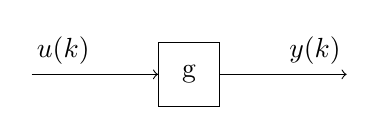
\begin{tikzpicture}[node distance=20mm, anchor=north]
\node[coordinate] (input) {};
\node[rectangle, draw, right of=input, inner sep=3mm] (lti) {g};
\node[coordinate, right of=lti] (output) {};
\draw[->] (input) -- node[near start, above] {$u(k)$}  (lti);
\draw[->] (lti) -- node[near end, above] {$y(k)$} (output);
\end{tikzpicture}
\end{center}

\[ y(k) = g \ast u = \sum_{n=0}^\infty g(n) u(k-n) \]

If input signal is a pulse (delta-function)
\begin{center}
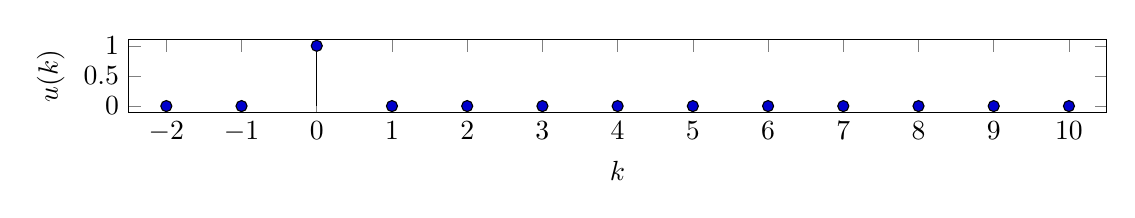
\begin{tikzpicture}
\begin{axis}[
  width=14cm,
  height=2.5cm,
  xlabel={$k$},
  ylabel={$u(k)$},
  xmin=-2.5,
  xmax=10.5,
]

\addplot+[black, ycomb, domain=-2:10, samples=13,variable=k] { (k==0)}; 

\end{axis}
\end{tikzpicture}
\end{center}

\vspace*{-5mm}
\[ y(k) = \sum_{n=0}^\infty g(n) \delta(k-n) = g(k) \]
\end{frame}

\begin{frame}[label=sec-1-2]{Linearity, time invariance and the pulse response}
The input signal

\begin{center}
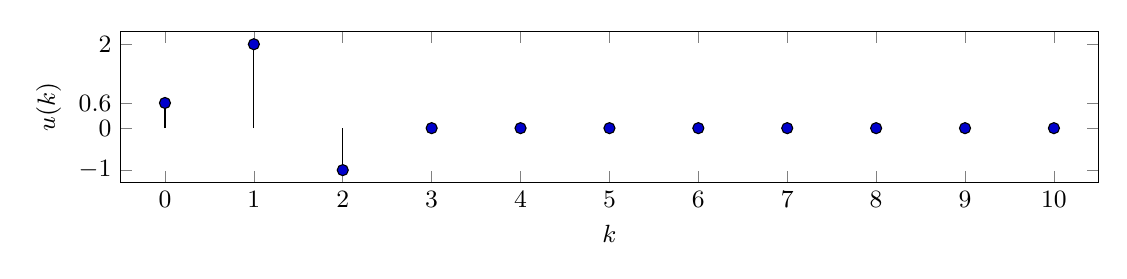
\begin{tikzpicture}
\small
\begin{axis}[
  width=14cm,
  height=3.5cm,
  xlabel={$k$},
  ylabel={$u(k)$},
  xmin=-0.5,
  xmax=10.5,
  ytick = {-1, 0, 0.6, 2},
]

\addplot+[black, ycomb, domain=-2:10, samples=13,variable=k] { 0.6*(k==0) + 2*(k==1) - 1*(k==2)}; 

\end{axis}
\end{tikzpicture}
\end{center}

\vspace*{-5mm}


Can be written 
\[u(k) = 0.6\delta(k) + 2\delta(k-1) - \delta(k-2) \]
Since the system's response to a pulse is given by $g(k)$, the output signal is
\[ y(k) = ?\]
\end{frame}

\begin{frame}[label=sec-1-3]{Linearity, time invariance and the pulse response}
The input signal

\begin{center}
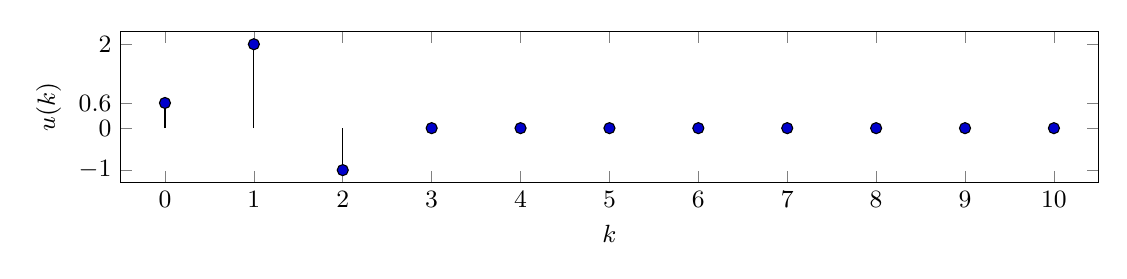
\begin{tikzpicture}
\small
\begin{axis}[
  width=14cm,
  height=3.5cm,
  xlabel={$k$},
  ylabel={$u(k)$},
  xmin=-0.5,
  xmax=10.5,
  ytick = {-1, 0, 0.6, 2},
]

\addplot+[black, ycomb, domain=-2:10, samples=13,variable=k] { 0.6*(k==0) + 2*(k==1) - 1*(k==2)}; 

\end{axis}
\end{tikzpicture}
\end{center}

\vspace*{-5mm}


Can be written 
\[u(k) = 0.6\delta(k) + 2\delta(k-1) - \delta(k-2) \]
Since the system's response to a pulse is given by $g(k)$, the output signal is
\[ y(k) = 0.6g(k) + 2g(k-1) - g(k-2) \]
\end{frame}


\begin{frame}[label=sec-1-4]{The output of a causal, linear discrete-time system is a weighted sum of previous input}
\[ y(k) = g \ast u = \sum_{n=0}^\infty g(n) u(k-n) \]
The \alert{weighting function} $g(k)$ is the \alert{pulse response} of the system.

What if the weighting function looks like this

\begin{center}
\begin{tikzpicture}
\small
\begin{axis}[
  width=14cm,
  height=3.5cm,
  xlabel={$k$},
  ylabel={$g(k)$},
  xmin=-0.5,
  xmax=10.5,
  ytick = {0, 1},
]

\addplot+[black, ycomb, domain=-2:10, samples=13,variable=k] { (k==4)}; 

\end{axis}
\end{tikzpicture}
\end{center}

\[y(k) = \]
\end{frame}

\begin{frame}[label=sec-1-5]{Exercise: Impulse response}
\end{frame}



\section{The shift operator}
\label{sec-2}
\begin{frame}[label=sec-2-1]{The shift operator}
\begin{itemize}
\item For difference equations the shift operator \(\shift\) is very useful.
\item The shift operator is defined for double-infinite sequences $x_k$, i.e. the sequence $x_k$ must be infinitely long both for negative and positive $k$.
\item The operator shifts the sequence ahead one step:
\[ \shift x_k = x_{k+1} \]
\end{itemize}
\end{frame}

\begin{frame}[label=sec-2-2]{The difference equation is a representation of a discrete-time dynamical systems}
\begin{center}
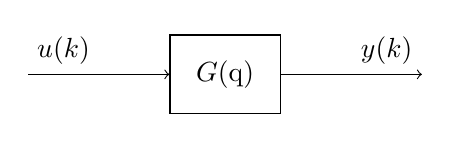
\begin{tikzpicture}[node distance=25mm]
\node[rectangle, draw, minimum height=10mm, minimum width=14mm] (sys) {$G(\shift)$};
\node[coordinate, left of=sys] (input) {};
\node[coordinate, right of=sys] (output) {};

\draw[->] (input) -- node [near start, above] {$u(k)$} (sys);
\draw[->] (sys) -- node [near end, above] {$y(k)$} (output);

\end{tikzpicture}
\end{center}

\[ y_{k+n} + a_1 y_{k+n-1} + \cdots + a_n y_k =  b_0 u_{k+m} + b_1 u_{k+m-1} + \cdots + b_m u_k \]

\[ \left( \shift^n + a_1 \shift^{n-1} + \cdots + a_n \right) y(k) = \left( b_0 \shift^m + b_1\shift^{m-1} + \cdots + b_m \right)  u(k) \]

\[ y(k) = \frac{b_0 \shift^m + b_1\shift^{m-1} + \cdots + b_m}{ \shift^n + a_1 \shift^{n-1} + \cdots + a_n} u(k) = \frac{B(\shift)}{A(\shift)} u(k) = G(\shift) u(k) \]
\end{frame}

\section{First order system and pulse response}
\label{sec-3}

\begin{frame}[label=sec-3-1]{First order systems}
\begin{center}
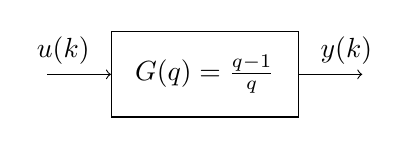
\begin{tikzpicture}[node distance=20mm, anchor=north]
\node[coordinate] (input) {};
\node[rectangle, draw, right of=input, inner sep=3mm] (lti) {$G(q)=\frac{q-1}{q}$};
\node[coordinate, right of=lti] (output) {};
\draw[->] (input) -- node[near start, above] {$u(k)$}  (lti);
\draw[->] (lti) -- node[near end, above] {$y(k)$} (output);
\end{tikzpicture}
\end{center}

The system with pulse-transfer operator $G(q)=\frac{q-1}{q}$ corresponds to the difference equation
\[ y(k) = G(q)u(k) \Leftrightarrow y(k) = \frac{q-1}{q} u(k) \]
\[ y(k+1) = ?\]
\end{frame}

\begin{frame}[label=sec-3-2]{First order systems}
\begin{center}
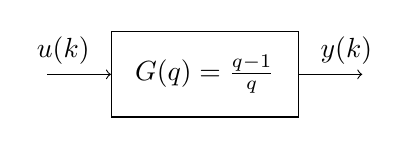
\begin{tikzpicture}[node distance=20mm, anchor=north]
\node[coordinate] (input) {};
\node[rectangle, draw, right of=input, inner sep=3mm] (lti) {$G(q)=\frac{q-1}{q}$};
\node[coordinate, right of=lti] (output) {};
\draw[->] (input) -- node[near start, above] {$u(k)$}  (lti);
\draw[->] (lti) -- node[near end, above] {$y(k)$} (output);
\end{tikzpicture}
\end{center}

The system with pulse-transfer operator $G(q)=\frac{q-1}{q}$ corresponds to the difference equation
\[ y(k) = G(q)u(k) \Leftrightarrow y(k) = \frac{q-1}{q} u(k) \]
\[ y(k+1) = u(k+1)-u(k), \quad \text{i.e.~a discrete-time differentiator}\]
\end{frame}

\begin{frame}[label=sec-3-3]{First order systems}
\begin{center}
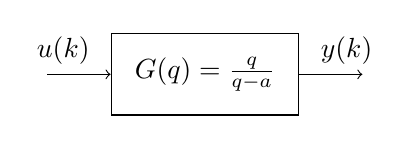
\begin{tikzpicture}[node distance=20mm, anchor=north]
\node[coordinate] (input) {};
\node[rectangle, draw, right of=input, inner sep=3mm] (lti) {$G(q)=\frac{q}{q-a}$};
\node[coordinate, right of=lti] (output) {};
\draw[->] (input) -- node[near start, above] {$u(k)$}  (lti);
\draw[->] (lti) -- node[near end, above] {$y(k)$} (output);
\end{tikzpicture}
\end{center}

The system with pulse-transfer operator $G(q)=\frac{q}{q-a}$ corresponds to the difference equation
\[ y(k) = G(q)u(k) \Leftrightarrow y(k) = \frac{q}{q-a} u(k) \]
\[ y(k+1) = ?\]
\end{frame}

\begin{frame}[label=sec-3-4]{First order systems}
\begin{center}
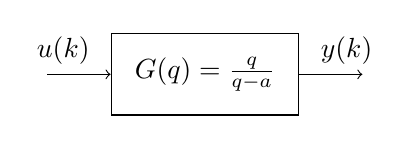
\begin{tikzpicture}[node distance=20mm, anchor=north]
\node[coordinate] (input) {};
\node[rectangle, draw, right of=input, inner sep=3mm] (lti) {$G(q)=\frac{q}{q-a}$};
\node[coordinate, right of=lti] (output) {};
\draw[->] (input) -- node[near start, above] {$u(k)$}  (lti);
\draw[->] (lti) -- node[near end, above] {$y(k)$} (output);
\end{tikzpicture}
\end{center}

The system with pulse-transfer operator $G(q)=\frac{q}{q-a}$ corresponds to the difference equation
\[ y(k) = G(q)u(k) \Leftrightarrow y(k) = \frac{q}{q-a} u(k) \]
\[ y(k+1) = ay(k) + u(k+1). \quad \text{If $a=1$, the system is a discrete-time integrator}\]
\end{frame}

\begin{frame}[label=sec-3-5]{Pulse-response of a first order system}
\[ y(k+1) = ay(k) + u(k+1) \]
\end{frame}

\begin{frame}[label=sec-3-6]{Pulse response of a first order system}
\[ y(k+1) = ay(k) + u(k+1) \]

Pair the pulse response to each of the values of $a$
\[ \text{I)}\; a=1 \qquad \text{II)}\; a=2 \qquad \text{III)}\; a = 0.5 \qquad \text{IV)}\; a=-0.9 \]

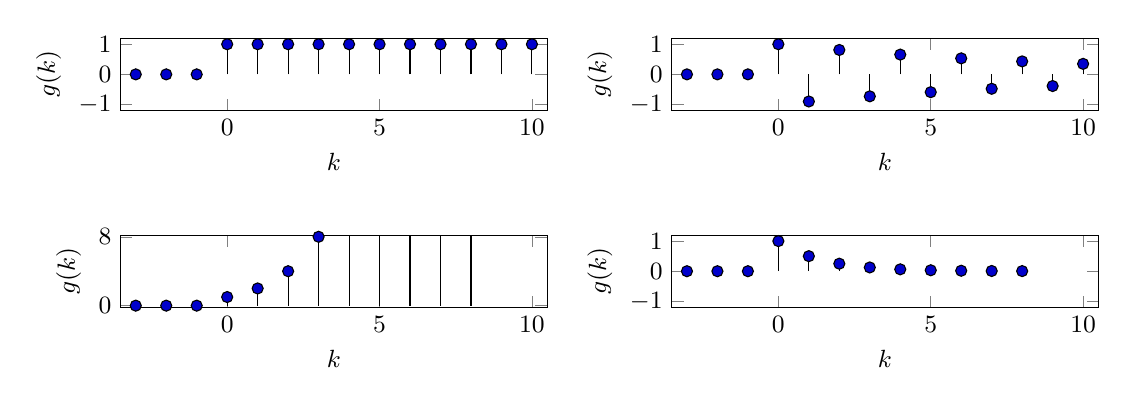
\begin{tikzpicture}
\small
\begin{axis}[
width=7cm,
height=2.5cm,
xlabel={$k$},
ylabel={$g(k)$},
xmin=-3.5,
xmax=10.5,
ytick = {-1,0,1},
ymin = -1.2, ymax=1.2,
]
\addplot+[black, ycomb, domain=-3:10, samples=14,variable=k] { (k>=0)*pow(1,k)};
\end{axis}

\begin{axis}[
xshift=7cm,
width=7cm,
height=2.5cm,
xlabel={$k$},
ylabel={$g(k)$},
xmin=-3.5,
xmax=10.5,
ytick = {0},
ytick = {-1,0,1},
ymin = -1.2, ymax=1.2,
]
\addplot+[black, ycomb, domain=-3:10, samples=14,variable=k] { (k>=0)*pow(-0.9,k)};
\end{axis}

\begin{axis}[
xshift=0cm,
yshift=-2.5cm,
width=7cm,
height=2.5cm,
xlabel={$k$},
ylabel={$g(k)$},
xmin=-3.5,
xmax=10.5,
ytick = {0},
ytick = {-1,0,8},
ymin = -0.2, ymax=8.2,
]
\addplot+[black, ycomb, domain=-5:8, samples=14,variable=k] {  (k>=0)*pow(2,k) };
\end{axis}

\begin{axis}[
xshift=7cm,
yshift=-2.5cm,
width=7cm,
height=2.5cm,
xlabel={$k$},
ylabel={$g(k)$},
xmin=-3.5,
xmax=10.5,
ytick = {0},
ytick = {-1,0,1},
ymin = -1.2, ymax=1.2,
]
\addplot+[black, ycomb, domain=-5:8, samples=14,variable=k] {  (k>=0)*pow(0.5,k)};
\end{axis}


\end{tikzpicture}
\end{frame}
% Emacs 25.3.50.2 (Org mode 8.2.10)
\end{document}